\documentclass[final,t]{beamer}
\mode<presentation>
{
%  \usetheme{Warsaw}
%  \usetheme{Aachen}
%  \usetheme{Oldi6}
%  \usetheme{I6td}
  \usetheme{I6dv}
%  \usetheme{I6pd}
%  \usetheme{I6pd2}
}
% additional settings
\setbeamerfont{itemize}{size=\normalsize}
\setbeamerfont{itemize/enumerate body}{size=\normalsize}
\setbeamerfont{itemize/enumerate subbody}{size=\normalsize}


\usepackage{algorithm}
\usepackage{algorithmic}


\usepackage{tikz}
\usetikzlibrary{calc}

% \newcommand{\theHalgorithm}{\arabic{algorithm}}

\usepackage{Definitions}
\usepackage{tensor}
\usepackage{empheq}
\usepackage{array}
\usepackage{color}
%\usepackage[usenames,dvipsnames,svgnames,table]{xcolor}
\usepackage{tikz}
\usetikzlibrary{calc}

% additional packages
\usepackage{times}
\usepackage{amsmath,amsthm, amssymb, latexsym}
\usepackage{exscale}

%\boldmath
\usepackage{booktabs, array}
%\usepackage{rotating} %sideways environment
\usepackage[english]{babel}
\usepackage[latin1]{inputenc}
%\usepackage[orientation=landscape,size=custom,width=200,height=120,scale=1.9]{beamerposter}
\usepackage[orientation=landscape,size=custom,width=121.92,height=91.44,scale=1.3]{beamerposter}
%\usepackage[orientation=landscape,size=custom,width=121,height=91,scale=1.3]{beamerposter}
\listfiles
\graphicspath{{figures/}}
% Display a grid to help align images
%\beamertemplategridbackground[1cm]

\title{\huge Nonparametric Estimation of Multi-View Latent Variable Models}
\author{Le Song, Animashree Anandkumar, Bo Dai and Bo Xie}
\institute[gt_cse]{Georgia Institute of Technology, University of California Irvine}
% \date[Aug. 31 , 2007]{Aug. 31 , 2007}


% abbreviations
\usepackage{xspace}
\makeatletter
\DeclareRobustCommand\onedot{\futurelet\@let@token\@onedot}
\def\@onedot{\ifx\@let@token.\else.\null\fi\xspace}
\def\eg{{e.g}\onedot} \def\Eg{{E.g}\onedot}
\def\ie{{i.e}\onedot} \def\Ie{{I.e}\onedot}
\def\cf{{c.f}\onedot} \def\Cf{{C.f}\onedot}
\def\etc{{etc}\onedot}
\def\vs{{vs}\onedot}
\def\wrt{w.r.t\onedot}
\def\dof{d.o.f\onedot}
\def\etal{{et al}\onedot}
\makeatother

%---------------------------------------------------------------------------------------------------
%---------------------------------------------------------------------------------------------------
%---------------------------------------------------------------------------------------------------
\begin{document}
\begin{frame}{} 
  \begin{columns}[t]
    %====================================================================================================
    \begin{column}{.3\linewidth}

      %---------------------------------------------------------------------------------------------------

      \begin{block}{Introduction}
        Given samples only from the \alert{observed variables} $\{X_t\}_{t\in[\ell] }$, could we recover the multi-view latent variable models generating the dataset?
        \begin{eqnarray*}
        \PP\rbr{\{X_t\}_{t \in [\ell]}}=\sum\nolimits_{h \in [k]} \PP(h) \cdot \prod\nolimits_{t \in [\ell]} \PP(X_t|h),\quad \alert{l\ge 3}
        \end{eqnarray*}
        where $h$ is \alert{discrete} and $\{X_t\}_{t\in[\ell] }$ are \alert{conditional independent} given $h$.
        \begin{figure}[h!]
        \centering
        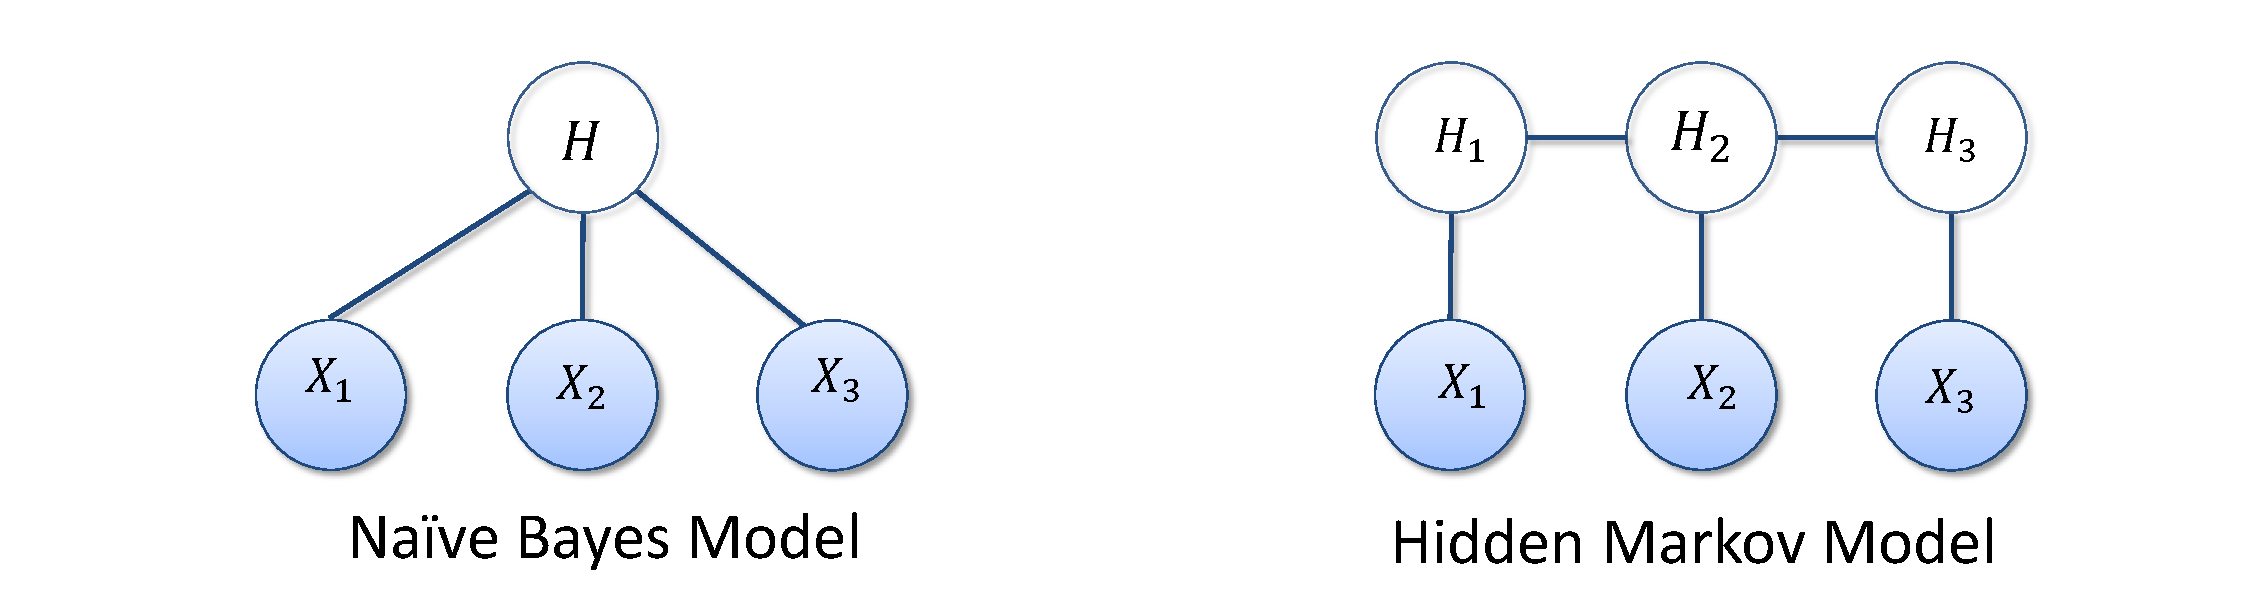
\includegraphics[width=\linewidth]{figures/example_mv.pdf} 
        \caption{Examples of multi-view latent variable models}
        \end{figure}
        
        We proposed a \alert{kernel} method for obtaining sufficient statistics for the model with \alert{theoretical guarantee}.
        \begin{itemize}
        \item Based on spectral algorithm for model estimation, our algorithm is \alert{computational efficient} and with \alert{provable guarantees}.
        \item \alert{Without the parametric assumption} involved in $\PP(X_t|h)$, our algorithm is more flexible and robust.
        \end{itemize}
      \end{block}
      \vspace{-0.5in}
      %---------------------------------------------------------------------------------------------------
      \begin{block}{Kernel Embeddings of Distributions}
        Denote $k(\cdot, \cdot)$ is the kernel function of a RKHS whose elements are functions $f:\Omega \mapsto \RR$ with
        inner product $\inner{\cdot}{\cdot}_{\Fcal}$. $k(x,\cdot)$ can be
        viewed as an implicit feature map $\phi(x)$ where $k(x, x') =
        \inner{\phi(x)}{\phi(x')}_{\Fcal}$

        A kernel embedding represents a density by its expected features,
        \begin{align*}
          \mu_{X} \, := \, \EE_{X} \sbr{\phi(X)} \, = \, \int_{\Xcal} \phi(x) \, d\PP(x)
        \end{align*}
        And the conditional distribution embedding is 
        $
          \mu_{X|h} \, := \, \EE_{X|h} \sbr{\phi(X)} 
        $.
        Kernel embeddings could be generalized to joint distribution of two or more variables using tensor product feature maps.
        \begin{eqnarray*}
            \Ccal_{X_{1:d}}
            := \EE_{X_{1:d}}\sbr{\otimes_{i=1}^d \phi(X_i)}
            = \int_{\Xcal^d} \rbr{\otimes_{i=1}^d \phi(x_i)}
            \,p(x_1,\ldots,x_d)\, \prod_{i=1}^d dx_i
        \end{eqnarray*}
        It could be viewed as a \alert{multi-linear operator} of order $d$ mapping
        from $\Fcal\times\ldots\times \Fcal$ to $\RR$. And thus,
        \begin{eqnarray*}
        \Ccal_{X_{1:d}} \times_1 f_1 \times_2 \ldots \times_d f_d := \inner{\Ccal_{X_{1:d}}}{\;\otimes_{i=1}^d f_d}_{\Fcal^d}
        =\EE_{X_{1:d}}\sbr{\prod_{i=1}^d \inner{\phi(X_i)}{f_i}_{\Fcal}}
        \end{eqnarray*}
      \end{block}
      \vspace{-0.5in}
      %---------------------------------------------------------------------------------------------------
      \begin{block}{Recap Multi-View Latent Variable Models}
      Tile these embeddings into a matrix, the conditional embedding operator is
      $
        \Ccal_{X|H} = \rbr{\mu_{X|h=1},\mu_{X|h=2},\ldots,\mu_{X|h=k}}
      $.

      Since we assume the hidden variable $H \in [k]$ is discrete, let $\pi_h:=\PP(h)$, then,
         \begin{align*}
         \Ccal_{HH} &= \EE_H[e_H \otimes e_H] = \rbr{
          \begin{array}{c}
            \pi_h \delta(h, h') \cr
          \end{array}
         }_{h,h' \in [l]},\\
         \Ccal_{HHH} &= \EE_H[e_H \otimes e_H \otimes e_H] 
          = \rbr{
          \begin{array}{c}
            \pi_h\ \delta(h,h')\ \delta(h',h'') \cr
          \end{array}
         }_{h,h',h''\in[l]}
        \end{align*}
      We obatin the factorization of $\PP(X_1,X_2)$ and $\PP(X_1,X_2,X_3)$ repsectively,
      \begin{eqnarray*}
        \Ccal_{X_1X_2}&=& \Ccal_{X|H}\, \Ccal_{HH}\, \Ccal_{X|H}^\top=\sum\nolimits_{h \in [k]} \pi_h\cdot \mu_{X|h} \otimes \mu_{X|h}\\
        \Ccal_{X_1 X_2 X_3} &=& \Ccal_{HHH} \times_1 \Ccal_{X|H} \times_2 \Ccal_{X|H} \times_3 \Ccal_{X|H}\\
        &=&\sum\nolimits_{h \in [k]} \pi_h\cdot \mu_{X|h} \otimes \mu_{X|h} \otimes \mu_{X|h}
      \end{eqnarray*}
      Under mild condition, the set $\{\pi_h, \mu_{X|h}\}$ is \alert{identifiable}.
      \end{block}

      \vspace{-0.5in}
    \end{column}


    %=====================================================================================================
    \begin{column}{.3\linewidth}
      %---------------------------------------------------------------------------------------------------


     \begin{block}{Spectral Algorithm}
          % \begin{algorithm}[t!]
          %For simplicity of exposition, the algorithm is explained for \alert{symmetric} view population case as if we could access the true opterator $\Ccal_{X_1 X_2}$ and $\Ccal_{X_1 X_2 X_3}$.
          For simplicity of exposition, the algorithm is explained for \alert{symmetric} view population case.
          \begin{itemize}
          \item[1.] Perform eigen-decomposition of $\Ccal_{X_1 X_2}$ which is rank $l$. Denote the $l$-leading eigenvectors be  $\Ucal_l:=(u_1,u_2,\ldots,u_l)$, and the eigen-value matrix be $S_l:=\diag(\sigma_1,\sigma_2,\ldots,\sigma_l)$. We have the whitening operator $\Wcal:= \Ucal_k S_k^{-1/2}$ which satisfies
          \begin{align*}
            \Wcal^\top \Ccal_{X_1X_2} \Wcal = (\Wcal^\top \Ccal_{X|H} \Ccal_{HH}^{1/2}) (\Ccal_{HH}^{1/2} \Ccal_{X|H}^\top \Wcal) = I
          \end{align*}
          and $M:=\Wcal^\top \Ccal_{X|H} \Ccal_{HH}^{1/2}$ is an orthogonal matrix.
          \item[2.] Apply the whiten operator to the 3rd order kernel embedding $\Ccal_{X_1 X_2 X_3}$
          \begin{eqnarray*}
            \Tcal := \Ccal_{X_1 X_2 X_3} \times_1 (\Wcal^\top) \times_2 (\Wcal^\top) \times_3 (\Wcal^\top)
            = \Ccal_{HHH}^{-1/2} \times_1 M \times_2 M \times_3 M,
          \end{eqnarray*}
          which is a tensor with orthogonal factors.
          \item[3.] Use tensor power method to find the leading $l$ eigenvectors $M$ for $\Tcal$. The corresponding $l$ eigenvalues $\lambda = (\lambda_1,\ldots,\lambda_l)^\top$ will then be equal to $(\PP(h=1)^{-1/2},\ldots,\PP(h=l)^{-1/2})$.
          \item[4.] Recover the conditional embedding operator by undoing the whitening step
          $
            \Ccal_{X|H} = (\Wcal^\top)^\dagger M \diag(\lambda).
          $
          \end{itemize}
      \vspace{-0.4in}
     \end{block}

      %-------------------------------------------------------------------------------------------------------

      %\begin{block}{Kernel Spectral Algorithm}
      \begin{block}{Kernelization}
      % We could carry all the computation above by \alert{kernel matrices}. 
      % For simplicity of exposition, the algorithm is explained for \alert{symmetric} view case.
      
      Given $m$ observations $\Dcal_{X_1 X_2 X_3}=\{(x_1^i,x_2^i,x_3^i)\}_{i \in [m]}$ drawn~\iid~from a multi-view latent variable model $\PP(X_1,X_2,X_3)$,  we denote the implicit feature matrix
      \vspace{-0.5in}
      \begin{align*}
        \Phi &:= (\phi(x_1^1), \ldots, \phi(x_1^m), \phi(x_2^1),  \ldots, \phi(x_2^m)),  \\
        \Psi &:= (\phi(x_2^1), \ldots, \phi(x_2^m), \phi(x_1^1),  \ldots, \phi(x_1^m)),
      \end{align*}
      and the corresponding kernel matrix by $K = \Phi^\top \Phi$ and $L = \Psi^\top \Psi$ respectively. 
      $
        \otimes\sbr{\xi_1,\xi_2,\xi_3} := \xi_1\otimes\xi_2\otimes\xi_3 + \xi_3\otimes\xi_1\otimes\xi_2 + \xi_2\otimes\xi_3\otimes\xi_1.
      $
      % Then, the estimated 2nd order embedding is $\widehat \Ccal_{X_1 X_2} = \frac{1}{2m} \Phi \Psi^\top$. 
      % \begin{itemize}
      % \item[{1.}] Since $\widehat \Ucal_k = \Phi (\beta_1,\ldots,\beta_k)$ with $\beta \in \RR^{2m}$, then, we could transform the eigen-decomposition of \alert{infinit} operator to \alert{kernel matrices}.
      % \begin{eqnarray*}
      % &&\widehat \Ccal_{X_1 X_2}\, \widehat \Ccal_{X_1 X_2}^\top\, u = \widehat \sigma^2 \;u
      % ~\Rightarrow~
      % \frac{1}{4m^2}\Phi \Psi^\top \Psi \Phi^\top \Phi \beta = \widehat \sigma^2 \,\Phi \beta \\
      % &~\Rightarrow~&
      % \frac{1}{4m^2} K L K \beta = \widehat \sigma^2 \,K \beta
      % ~\Rightarrow~ \frac{1}{4m^2} R L R^\top \widetilde{\beta} =\widehat  \sigma^2 \, \widetilde{\beta}.
      % \end{eqnarray*}
      % where the Cholsky decomposition of $K$ be $R^\top R$ and $\widetilde{\beta}=R\beta$.
      % \item[{2.}] Whitten the empirical 3rd order embedding
      % $
      %   &\widehat \Ccal_{X_1 X_2 X_3}:= \frac{1}{3m}\sum\nolimits_{i=1}^{m} \otimes \sbr{\phi(x_1^i), \phi(x_2^i), \phi(x_3^i)}
      % $
      % using $\widehat \Wcal:= \widehat \Ucal_k \widehat S_k^{-1/2}$, and,
      % $        \widehat \Tcal := \frac{1}{3m}\sum\nolimits_{i=1}^m \otimes\sbr{\xi(x_1^i), \xi(x_2^i), \xi(x_3^i)}, 
      %   \xi(x_1^i) := \widehat S_k^{-1/2} (\beta_1,\ldots,\beta_k)^\top K_{:x_1^i}.
      % $
      % \item[{3.}] Run tensor power method on the \alert{finite dimension tensor} on $\widehat \Tcal$ to obtain its leading $l$ eigenvectors $\widehat M:=(\widehat v_1,\ldots,\widehat v_l)$ and the corresponding eigenvalues $\widehat \lambda := (\widehat\lambda_1,\ldots,\widehat\lambda_l)^\top$.
      % \item[{4.}] The estimates of the conditional embeddings are
      % \begin{align*}
      %   \widehat \Ccal_{X|H} = \Phi (\beta_1,\ldots,\beta_k) \widehat  S_k^{1/2} \widehat M \diag(\widehat \lambda).
      % \end{align*}
      % \end{itemize}
      % \end{block}
      % \vspace{-0.2in}
      % %------------------------------------------------------------------------------------------
      % \begin{block}{Algorithm Summary}
          \vspace{-2mm}
          \begin{center}
          \hline
          \hline
          \vspace{2mm}
          \textbf{Kernel Spectral Algorithm}\\
          %\vspace{-4mm}
          \hline
          \end{center}
          \textbf{In}: Kernel matrices $K$ and $L$, and desired rank $k$ \\
          \textbf{Out}: A vector $\widehat \pi \in \RR^k$ and a matrix $A \in \RR^{2m\times k}$\\[-0.4cm]
          \begin{algorithmic}[1]
            \STATE Cholesky decomposition:\ $K=R^\top R$
            \STATE Eigen-decomposition:\ $\frac{1}{4m^2} R L R^\top \widetilde{\beta} = \widehat \sigma^2\,\widetilde{\beta}$
            \STATE Use $k$ leading eigenvalues:\ $\widehat S_k = \diag(\widehat \sigma_1,\ldots,\widehat \sigma_k)$
            \STATE Use $k$ leading eigenvectors $(\widetilde{\beta}_1,\ldots,\widetilde{\beta}_k)$ to
            compute:\ $(\beta_1,\ldots,\beta_k) = R^\dagger (\widetilde{\beta}_1,\ldots,\widetilde{\beta}_k)$
            \STATE Form tensor: $\widehat \Tcal = \frac{1}{3m}\sum\nolimits_{i=1}^m \otimes\sbr{\xi(x_1^i), \xi(x_2^i), \xi(x_3^i)}$ where $\xi(x_1^i) = \widehat S_k^{-1/2} (\beta_1,\ldots,\beta_k)^\top K_{:x_1^i}$
            \STATE Power method: eigenvectors $\widehat M:=(\widehat v_1,\ldots,\widehat v_k)$, and the eigenvalues $\widehat \lambda := (\widehat\lambda_1,\ldots,\widehat\lambda_k)^\top$ of $\widehat \Tcal$
            \STATE $A = (\beta_1,\ldots,\beta_k) \widehat  S_k^{1/2} \widehat M \, \diag(\widehat \lambda)$
            \STATE $\widehat \pi = (\widehat\lambda_1^{-2},\ldots,\widehat\lambda_k^{-2})^\top$
          \end{algorithmic}
          \hline
          \vspace{-0.15in}
     \end{block}


    %------------------------------------------------------------------------------------------
    \begin{block}{Illustration}
    Illustration of the performance on Gaussians/Gamma mixtures.
    \begin{center}
        \begin{tabular}{cc}
        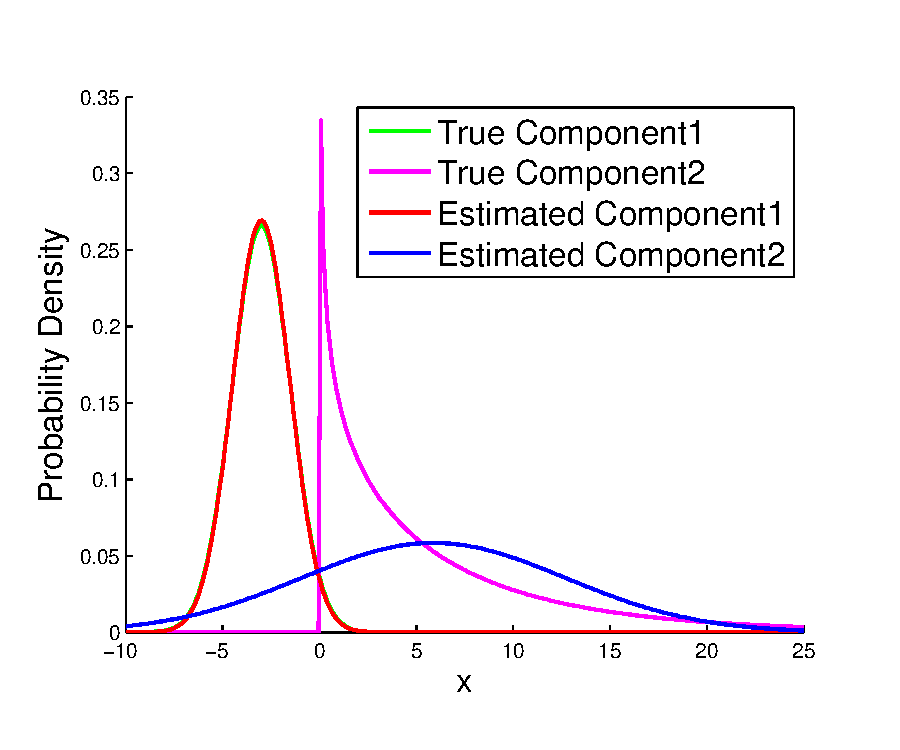
\includegraphics[width=0.4\textwidth]{../experiment/visualization/em_visual_k_2_view_1-crop}&
        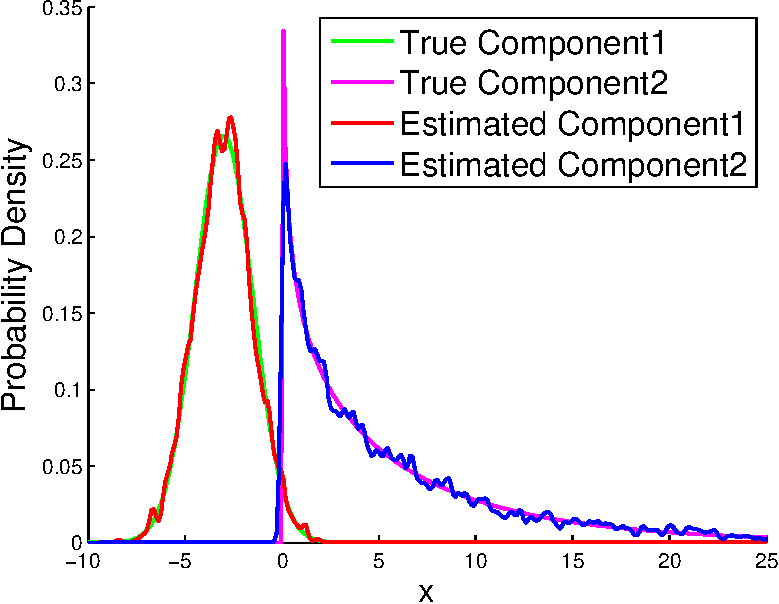
\includegraphics[width=0.4\textwidth]{../experiment/visualization/visual_k_2_view_1-crop-crop}\\
        (a) GMM & (b) Kernel Spectral Algorithm
        \end{tabular}
    \end{center}
    \vspace{-0.4in}
    \end{block}

    \end{column}

    %===========================================================================================
    \begin{column}{0.3\linewidth}
      %-----------------------------------------------------------------------------------------
      \begin{block}{Sample Complexity}
      \textbf{Theorem}
        \emph{Pick  any $\delta\in (0,1)$. When the number of samples $m$ satisfies
        $ m >\frac{\theta\rho^2  \log\frac{2}{\delta}}{\sigma^2_k(\Ccal_{X_1 X_2})},
        \quad \theta:= \max\left(\frac{C_3 k^2 \rho}{\sigma_k( \Ccal_{X_1 X_2})}, \frac{C_4k^{2/3}\iffalse(1+\sigma_{k+1}(\Ccal_{X_1 X_2}))^2 \fi }{\pi_{\min}^{1/3}}\right)$, for some constants $C_3, C_4>0$, and the number of iterations $N$  and  the number of random initialization vectors $L$  (drawn uniformly on the sphere $\mathcal{S}^{k-1}$)  satisfy
        $$
          N \geq C_2 \cdot \biggl( \log(k) + \log\log\Bigl(
         \frac{1}{\sqrt{\pi_{\min}}\epsilon_{\Tcal}} \Bigr) \biggr),
        $$
        for constant $C_2>0$ and  $L = \poly(k) \log(1/\delta)$,  the robust power method yields eigen-pairs $(\h{\lambda}_i, \h{v}_i)$ such that there exists a permutation $\eta$, with probability $1-4\delta$, we have
        \begin{align*}
        &\|\pi^{-1/2}_{j} \mu_{X|h=j}-(\beta_1,\ldots,\beta_k) \widehat  S_k^{1/2}\h{v}_{\eta(j)}\|_{\Fcal} \leq 8 \epsilon_{\Tcal} \cdot\pi^{-1/2}_{j}
        , \\
        &|\pi^{-1/2}_{j}-\h{\lambda}_{\eta(j)}| \leq  5\epsilon_{\Tcal}, \quad \forall j \in [k],
        \end{align*}
        % \begin{align*}
        % &\|\pi^{-1/2}_{j} \mu_{X|h=j}-\h{v}_{\eta(j)}\|_{\Fcal} \leq 8 \epsilon_{\Tcal} \cdot\pi^{-1/2}_{j}
        % , \\
        % &|\pi^{-1/2}_{j}-\h{\lambda}_{\eta(j)}| \leq  5\epsilon_{\Tcal}, \quad \forall j \in [k],
        % \end{align*}
        and $\|\Tcal - \sum\nolimits_{j=1}^k \hat\lambda_j \hat{\phi}_j^{\otimes 3} \| \leq 55\eps_{\Tcal}$ where $\eps_{\Tcal}:= \|\h{\Tcal} - \Tcal\|$ is the tensor perturbation bound
        \vspace{-10mm}
        \begin{align*} \eps_{\Tcal} \leq
        \frac{8 \rho^{1.5} \sqrt{\log\frac{2}{\delta}}}{\sqrt{m} \, \sigma_k^{1.5}(\Ccal_{X_1 X_2})} + \frac{512 \sqrt{2} \rho^3 \left(\log\frac{2}{\delta}\right)^{1.5}}{m^{1.5} \,\sigma_k^{3}(\Ccal_{X_1 X_2}) \sqrt{\pi_{\min}}}
        \end{align*}
        }
        {\bf Remark:} We note that the sample complexity is  $\poly(k, \rho, 1/\pi_{\min}, 1/\sigma_k(\Ccal_{X_1 X_2}))$ of a low order, and in particular,  it is $O(k^2)$, when the other parameters are fixed. 
      \end{block}


    %------------------------------------------------------------------------------------------
    \begin{block}{Synthetic Data: Model Estimation}
      \vspace{0.1in}
      We measured the performance of algorithms by the weighted $\ell_2$ norm difference
      $
      \sum_{h=1}^{k} \pi_h\, \sqrt{\sum_{j=1}^{m'} (p(x^j|h) - \widehat{p}(x^j|h))^2 },
      $
      %where $\{x^j\}_{j\in[m]}$ is a set of uniformly-spaced test points.
      \begin{center}
        \begin{tabular}{cccc}
          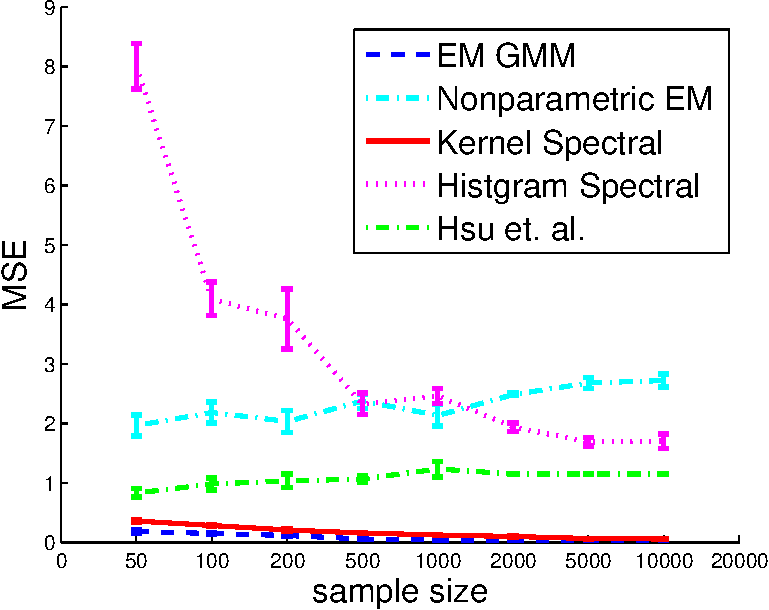
\includegraphics[width=0.23\textwidth]{../experiment/figure_new/sp_diff_gauss_k_2_view_2-crop} &
          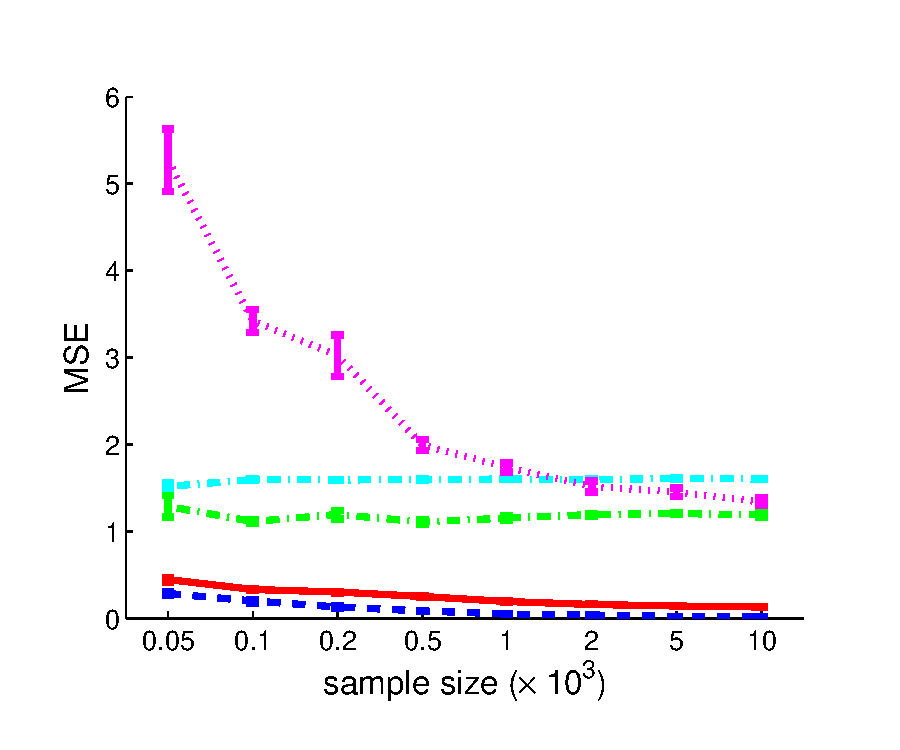
\includegraphics[width=0.23\textwidth]{../experiment/figure_new/sp_diff_gauss_k_3_view_3-crop} &
          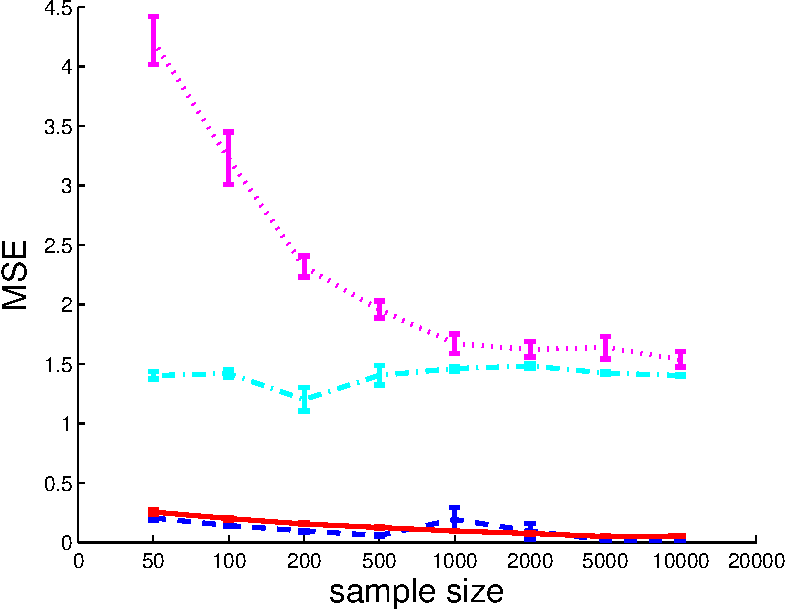
\includegraphics[width=0.23\textwidth]{../experiment/figure_new/sp_diff_gauss_k_4_view_1-crop} &
          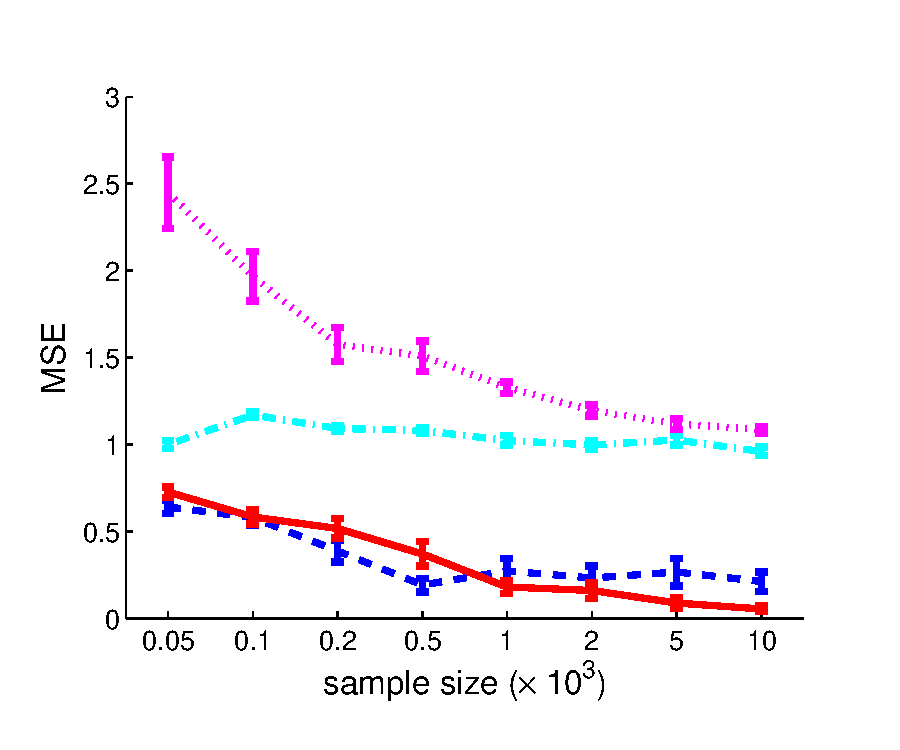
\includegraphics[width=0.23\textwidth]{../experiment/figure_new/sp_diff_gauss_k_8_view_1-crop} \\[-1mm]
          (a) $k=2$ & (b) $k=3$ & (c) $k=4$ & (d)$k=8$ \\[-1mm]
          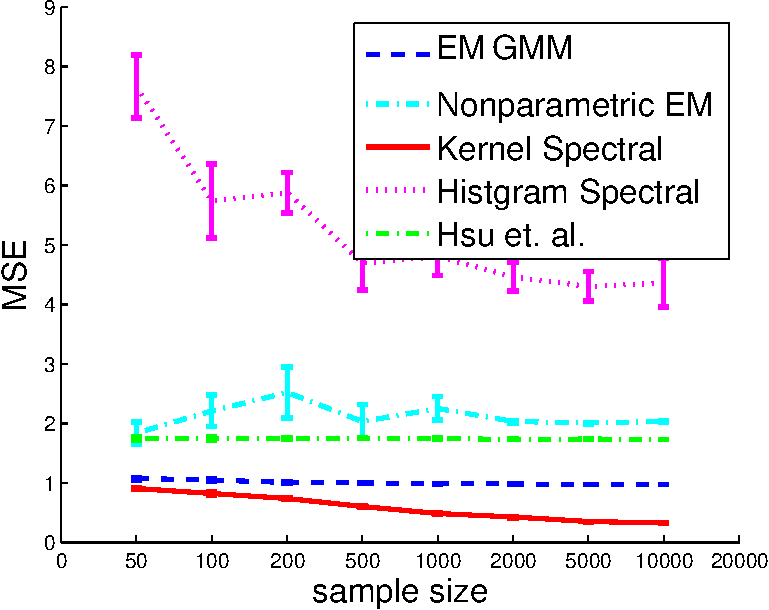
\includegraphics[width=0.23\textwidth]{../experiment/figure_new/sp_diff_heter_k_2_view_2-crop} &
          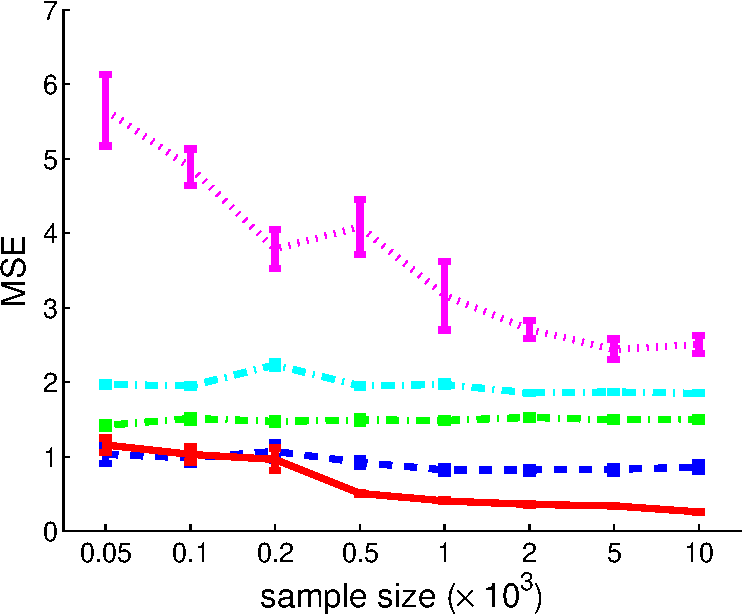
\includegraphics[width=0.23\textwidth]{../experiment/figure_new/sp_diff_heter_k_3_view_3-crop} &
          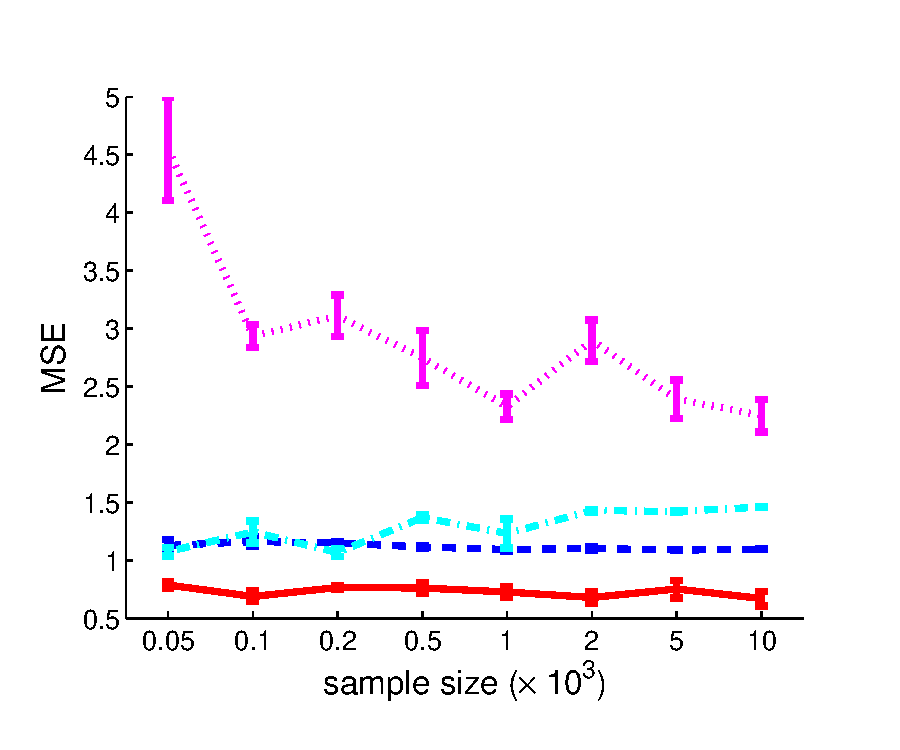
\includegraphics[width=0.23\textwidth]{../experiment/figure_new/sp_diff_heter_k_4_view_1-crop} &
          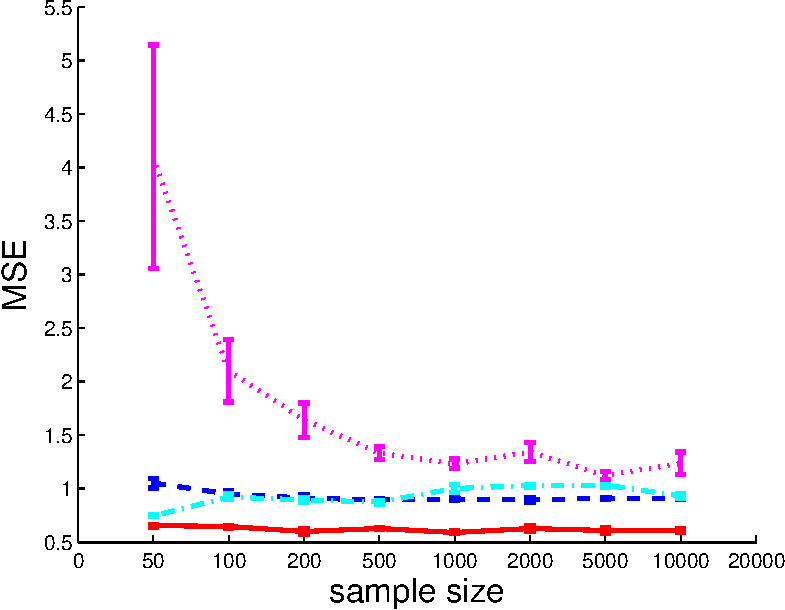
\includegraphics[width=0.23\textwidth]{../experiment/figure_new/sp_diff_heter_k_8_view_1-crop} \\[-1mm]
          (e) $k=2$ & (f) $k=3$ & (g)  $k=4$ & (h) $k=8$ \\[-1mm]
        \end{tabular}
        \vspace{-2mm}
        \caption{(a)-(d) Mixture of Gaussian distributions with $k=2,3,4,8$. (e)-(h) Mixture of Gaussian/Gamma distribution with $k=2,3,4,8$. }
      \end{center}
      % \begin{figure}
      %   \centering
      %   \begin{subfigure}
      %         \includegraphics[width=0.2\columnwidth]{figures/ground_truth_3d1.pdf}
      %         \caption{Ground truth}
      %   \end{subfigure}
      %   \begin{subfigure}
      %         \includegraphics[width=0.2\columnwidth]{figures/kde_3d1.pdf}
      %         \caption{Ordinary KDE}
      %   \end{subfigure}
      %   \begin{subfigure}
      %         \includegraphics[width=0.2\columnwidth]{figures/spkhmm_3d1.pdf}
      %         \caption{Kernel Spectral HMM}
      %   \end{subfigure}
      %   \begin{subfigure}
      %         \includegraphics[width=0.2\columnwidth]{figures/spkde_3d1.pdf}
      %         \caption{Low Rank KDE}
      %   \end{subfigure}
      % \end{figure}
    \vspace{-0.3in}
    \end{block}

    %----------------------------------------------------------------------------------------------
    \begin{block}{Real-World Data: Clustering Task}
      We experimented with clustering on flow cyntometry datasets. %We evaluated the clustering performance using f-score. 
      \begin{center}
      \begin{tabular}{c}
        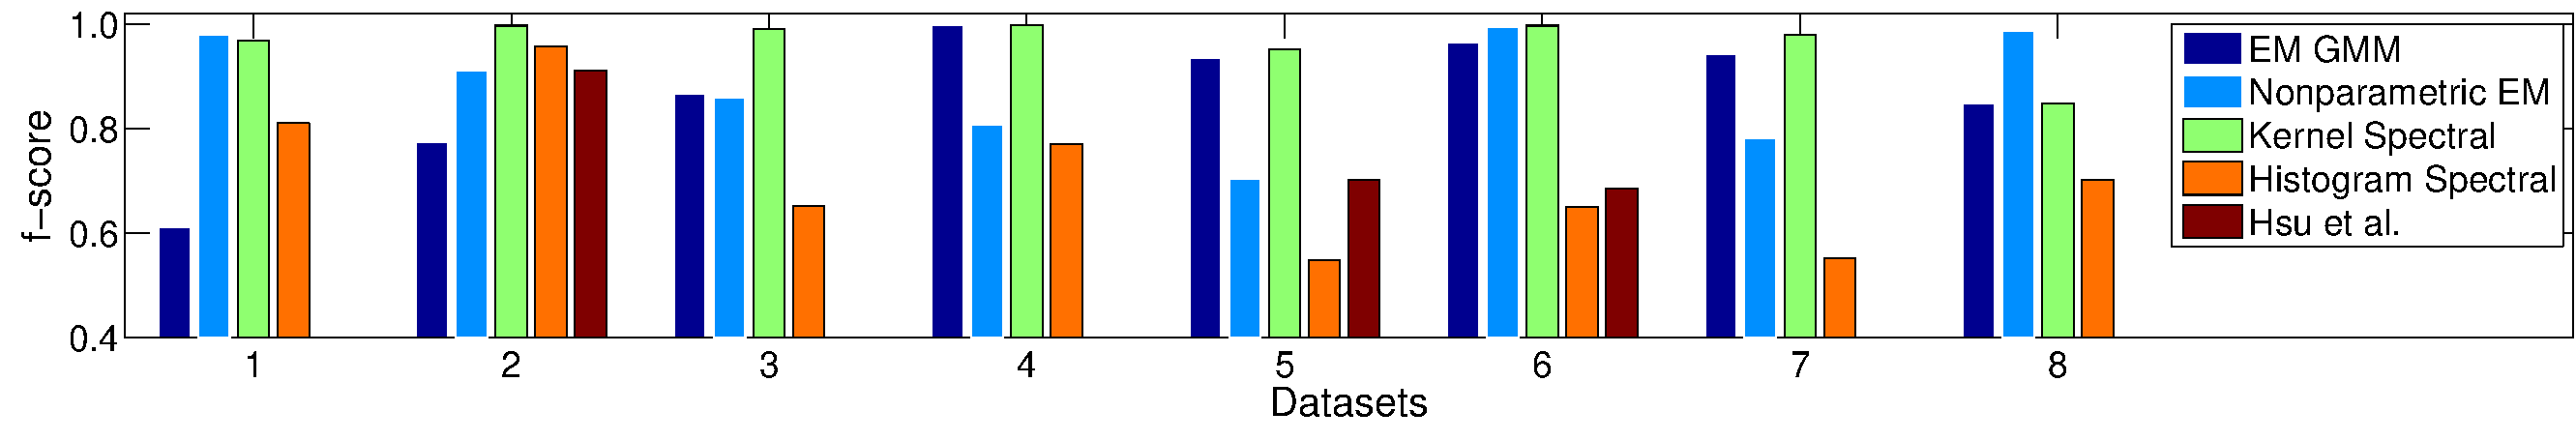
\includegraphics[width=0.82\textwidth]{../experiment/figure_new/paired_bar_chat_k_2} \\[-2mm]
        (a) number of clusters $k=2$ \\[-1mm]
        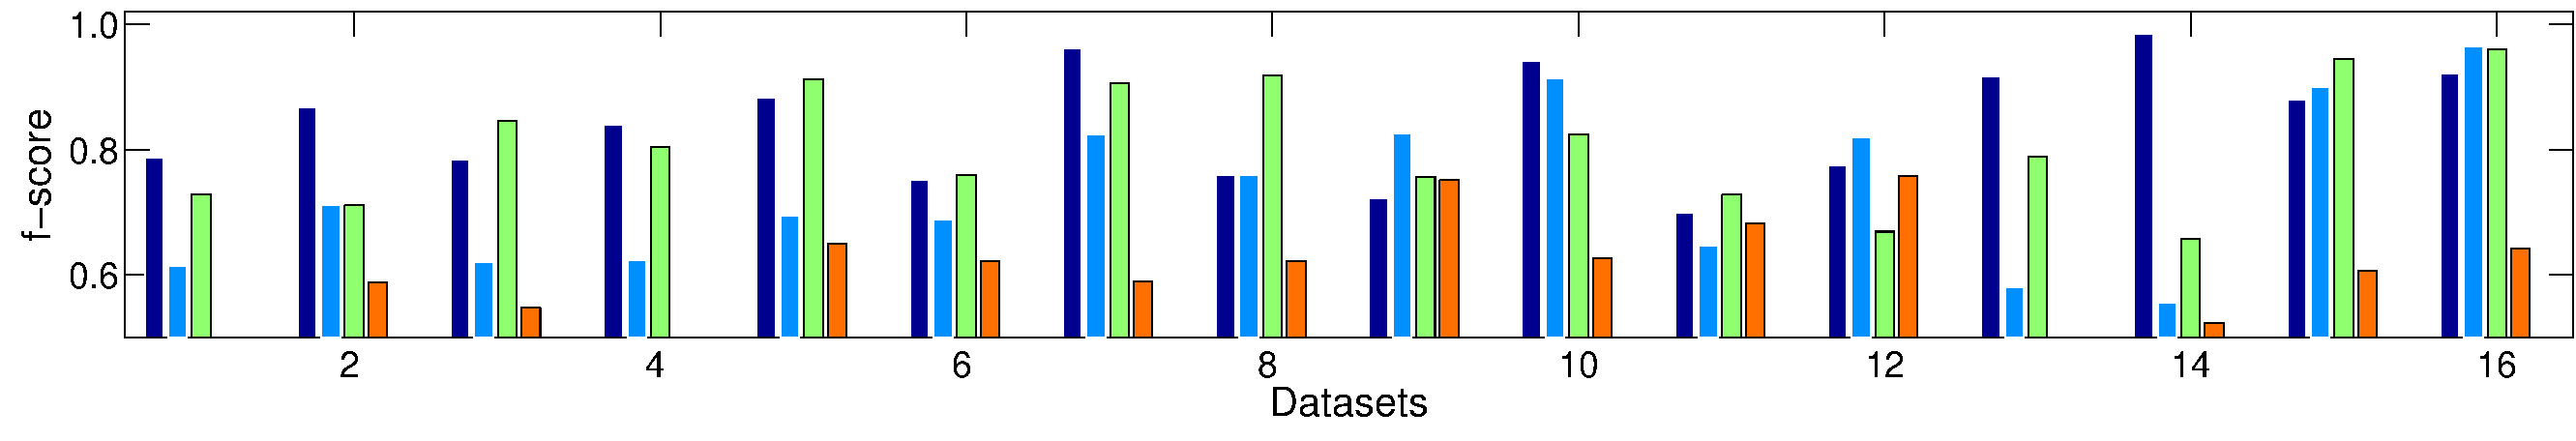
\includegraphics[width=0.98\textwidth]{../experiment/figure_new/paired_bar_chat_k_3}  \\[-2mm]
        (b) number of clusters $k=3$
      \end{tabular}
      \vspace{-4mm}
      \caption{Clustering results on the DLBCL flow cytometry datasets.}
      \vspace{-3mm}
      \end{center}
    \end{block}
    \end{column}

  \end{columns}
\end{frame}

\end{document}


%%%%%%%%%%%%%%%%%%%%%%%%%%%%%%%%%%%%%%%%%%%%%%%%%%%%%%%%%%%%%%%%%%%%%%%%%%%%%%%%%%%%%%%%%%%%%%%%%%%%
%%% Local Variables: 
%%% mode: latex
%%% TeX-PDF-mode: t
%%% End: 